\begin{figure}[htb]
\centering
\includegraphics[page=6,width=0.33\textwidth]{\FCNCFigures/xTFW/showFake/NOMINAL/reg2mtau1b3jos_vetobtagwp70_highmet/BDTG_test.pdf}
\put(-30, 80){\textbf{(a)}}
\includegraphics[page=6,width=0.33\textwidth]{\FCNCFigures/xTFW/showFake/NOMINAL/reg2mtau1b3jos_vetobtagwp70_highmet/chi2.pdf}
\put(-30, 80){\textbf{(b)}}
\includegraphics[page=6,width=0.33\textwidth]{\FCNCFigures/xTFW/showFake/NOMINAL/reg2mtau1b3jos_vetobtagwp70_highmet/dphitauetmiss.pdf}
\put(-30, 80){\textbf{(c)}}
\\
\includegraphics[page=6,width=0.33\textwidth]{\FCNCFigures/xTFW/showFake/NOMINAL/reg2mtau1b3jos_vetobtagwp70_highmet/drtaujmin.pdf}
\put(-30, 80){\textbf{(d)}}
\includegraphics[page=6,width=0.33\textwidth]{\FCNCFigures/xTFW/showFake/NOMINAL/reg2mtau1b3jos_vetobtagwp70_highmet/drtautau.pdf}
\put(-30, 80){\textbf{(e)}}
\includegraphics[page=6,width=0.33\textwidth]{\FCNCFigures/xTFW/showFake/NOMINAL/reg2mtau1b3jos_vetobtagwp70_highmet/etmiss.pdf}
\put(-30, 80){\textbf{(f)}}
\\
\includegraphics[page=6,width=0.33\textwidth]{\FCNCFigures/xTFW/showFake/NOMINAL/reg2mtau1b3jos_vetobtagwp70_highmet/phicent.pdf}
\put(-30, 80){\textbf{(g)}}
\includegraphics[page=6,width=0.33\textwidth]{\FCNCFigures/xTFW/showFake/NOMINAL/reg2mtau1b3jos_vetobtagwp70_highmet/t1mass.pdf}
\put(-30, 80){\textbf{(h)}}
\includegraphics[page=6,width=0.33\textwidth]{\FCNCFigures/xTFW/showFake/NOMINAL/reg2mtau1b3jos_vetobtagwp70_highmet/t1vismass.pdf}
\put(-30, 80){\textbf{(i)}}
\\
\includegraphics[page=6,width=0.33\textwidth]{\FCNCFigures/xTFW/showFake/NOMINAL/reg2mtau1b3jos_vetobtagwp70_highmet/t2mass.pdf}
\put(-30, 80){\textbf{(j)}}
\includegraphics[page=6,width=0.33\textwidth]{\FCNCFigures/xTFW/showFake/NOMINAL/reg2mtau1b3jos_vetobtagwp70_highmet/t2vismass.pdf}
\put(-30, 80){\textbf{(k)}}
\includegraphics[page=6,width=0.33\textwidth]{\FCNCFigures/xTFW/showFake/NOMINAL/reg2mtau1b3jos_vetobtagwp70_highmet/tau_pt_0.pdf}
\put(-30, 80){\textbf{(l)}}
\\
\caption{ The variables distributions for the background and merged tuH signal in the TTH $\thadhad$}
\label{fig:var_reg2mtau1b3jos_vetobtagwp70_highmet_1}
\end{figure}
\begin{figure}[htb]
\centering
\includegraphics[page=6,width=0.33\textwidth]{\FCNCFigures/xTFW/showFake/NOMINAL/reg2mtau1b3jos_vetobtagwp70_highmet/tau_pt_1.pdf}
\put(-30, 80){\textbf{(a)}}
\includegraphics[page=6,width=0.33\textwidth]{\FCNCFigures/xTFW/showFake/NOMINAL/reg2mtau1b3jos_vetobtagwp70_highmet/tautaumass.pdf}
\put(-30, 80){\textbf{(b)}}
\includegraphics[page=6,width=0.33\textwidth]{\FCNCFigures/xTFW/showFake/NOMINAL/reg2mtau1b3jos_vetobtagwp70_highmet/tautauvispt.pdf}
\put(-30, 80){\textbf{(c)}}
\\
\includegraphics[page=6,width=0.33\textwidth]{\FCNCFigures/xTFW/showFake/NOMINAL/reg2mtau1b3jos_vetobtagwp70_highmet/ttvismass.pdf}
\put(-30, 80){\textbf{(d)}}
\includegraphics[page=6,width=0.33\textwidth]{\FCNCFigures/xTFW/showFake/NOMINAL/reg2mtau1b3jos_vetobtagwp70_highmet/wmass.pdf}
\put(-30, 80){\textbf{(e)}}
\includegraphics[page=6,width=0.33\textwidth]{\FCNCFigures/xTFW/showFake/NOMINAL/reg2mtau1b3jos_vetobtagwp70_highmet/x1fit.pdf}
\put(-30, 80){\textbf{(f)}}
\\
\includegraphics[page=6,width=0.33\textwidth]{\FCNCFigures/xTFW/showFake/NOMINAL/reg2mtau1b3jos_vetobtagwp70_highmet/x2fit.pdf}
\put(-30, 80){\textbf{(g)}}
\caption{ The variables distributions for the background and merged tuH signal in the TTH $\thadhad$}
\label{fig:var_reg2mtau1b3jos_vetobtagwp70_highmet}
\end{figure}
